% !TeX spellcheck = en_GB

\documentclass[thesis=M,english,hidelinks]{FITthesis}[2018/03/12]

\usepackage[utf8]{inputenc}

\usepackage{graphicx}

\usepackage{dirtree}

\usepackage{amsmath} % maths

\department{Department of Theoretical Computer Science}
\title{Exploring use of non-negative matrix factorization for lossy audio compression}
\authorGN{Tomáš} %author's given name/names
\authorFN{Drbota} %author's surname
\author{Tomáš Drbota} %author's name without academic degrees
\authorWithDegrees{Bc. Tomáš Drbota} %author's name with academic degrees
\supervisor{doc. Ing. Ivan Šimeček, Ph.D.}
\acknowledgements{TODO}
\abstractEN{Non-negative matrix factorization has been successfully applied in various scenarios, mostly for analyzing large chunks of data and finding patterns in them for later use. Due to the nature of NMF, it has also seen some use in the field of image compression.

The purpose of this thesis is to research possible uses of non-negative matrix factorization in the problem of audio compression. A reference audio encoder and decoder using NMF will be implemented and various experiments using this encoder will be conducted. The results will be measured and compared to existing audio compressing solutions.}
\abstractCS{TODO}
\placeForDeclarationOfAuthenticity{Prague}
\keywordsCS{TODO}
\keywordsEN{lossy, audio, compression, processing, nmf, encoding}
\declarationOfAuthenticityOption{5}
% \website{http://site.example/thesis} %optional thesis URL

\begin{document}

\setsecnumdepth{part}
\chapter{Introduction}
In today's age of smartphones and other portable electronic devices capable of connecting to the internet, nearly everyone has access to a huge library of various media, including music and other audio. However, to transmit or store all of this data in its raw uncompressed form, a large amount of bandwidth and storage would be required. It is for that reason that we must employ some sort of compression.

Lossy audio codecs such as MP3, AAC, AC3, Vorbis, Opus etc. have been prevalent in this field as they are capable of compressing an audio signal into even a tenth of its size, without a perceivable difference in quality (to our ears, at least).

As such, this thesis will look into using Non-negative matrix factorization as a possible method for lossy compression of audio. It has been employed before for audio analysis, but works describing its applications for compression of audio specifically are limited.

First, we will have a look at what even is digital audio and important terms surrounding it. We will explore how it works, how is it recorded and stored in a computer and also what concerns go into analysing and compressing it.

Then, in chapter 3, non-negative matrix factorization is defined and described. We will talk about what it is, what is it realistically used for, how to use and implement it, and lastly its applications in the field of digital audio.

After that, we finally get to data compression. State of the art lossy audio codecs will be examined along with some lossless encodings that will be necessary later. Existing research into audio compression using NMF will also be summarized.

In chapters 5 and 6, I design and implement an NMF encoder and decoder (called ANMF). There are three different variants depending on what's being compressed - \emph{ANMF-RAW} for encoding raw audio, and \emph{ANMF-MDCT} along with \emph{ANMF-STFT} for encoding properly pre-processed audio. The file structure along with all the implementational details including used libraries will be described in great detail.

And finally, we take the implementation and evaluate the results. Using GstPEAQ as an objective measuring method, we compare our implementation to some of the reference codecs, namely MP3 and Opus, and draw conclusions from the results.


\addtocontents{toc}{\setcounter{tocdepth}{2}}

\setsecnumdepth{all}
\part{Background}
\chapter{Digital audio}
Sound as we know it can be defined as a physical wave travelling through air or another means. \cite{you_2010} It can be measured as change in air pressure surrounding an object. Once we have this electrical representation of the wave, we can convert it back and consequently play using speakers.

In the real world, these sound waves are generally composed of many different kinds of waves, with differing frequencies and amplitudes. The human ear can tell the difference between high (whistling) and low frequencies (drums), and knowledge of this will be useful later when we are discussing audio encoding.

\begin{figure}[ht]
	\label{fig:audio_signal}
	\caption[Example audio signal]{An example of an audio signal represented in PCM form.}
	\centering
	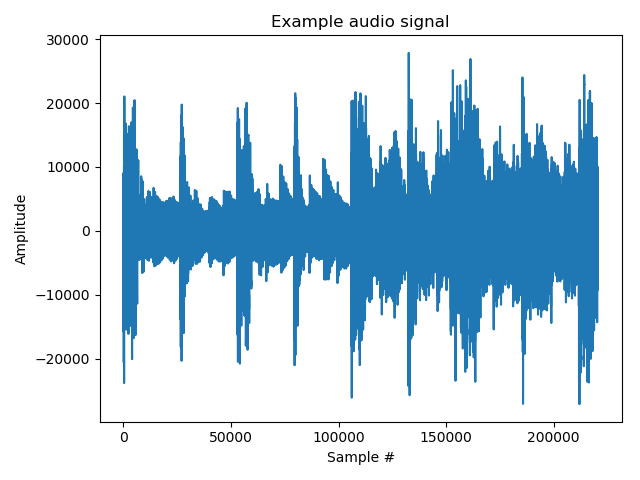
\includegraphics[width=\textwidth]{audio_signal.png}
\end{figure}

\section{Notation}
Below is a summary of the notation this chapter will be using.

\begin{table}[htbp]\caption{Digital audio notation}
\begin{tabular}{r l}
$t$ & symbol representing a time value in seconds \\
$\tau$ & symbol representing a "slow" time, time index with a lower resolution than $t$ \\
$\xi$ & symbol representing a frequency value in hertz \\
$x(t)$ & function representing the amplitude of a continuous signal at a time $t$ \\
$x_n$ & sequence representing the amplitude of a discrete signal indexed by $n$ \\
$w(t)$ & continuous windowing function at a time $t$ \\
$w_n$ & discrete windowing function indexed by $n$ \\
%$X(\xi)$ & function representing the frequency component of a signal for a frequency $\xi$ \\
$S(\xi)$ & the Fourier transform of a continuous signal \\
$S_k$ & the discrete Fourier transform of a discrete signal \\
$S(\tau, \xi)$ & the short-time Fourier transform of a continuous signal \\
$S_{k, \xi}$ & the discrete short-time Fourier transform of a discrete signal \\
$M_k$ & the Modified discrete cosine transform of a discrete signal
\end{tabular}
\end{table}

\section{Important terms}
.. TODO ..
sampling
nyquist frequency/limit
quantization
transient
aliasing
spectral leakage
windowing

\section{Digital audio representation}
Most commonly, the amount of air pressure is sampled many times a second and after being processed this information is stored as a discrete-time signal using numerical representations - this is what's known as a \emph{digital audio signal}. This entire process is called \emph{digital audio encoding}.

By sampling the audio signal, we will potentially be losing out on some information, but given a high enough sampling rate, the result will be imperceptible to the human ear. For general purpose audio and music, the standard sampling rate is 48 kHz, alternatively 44.1 kHz from the compact disk era.

Once we have our digital signal, there are two distinct kinds of ways we can represent, or, encode it. Both of them have many different data models for encoding \cite{you_2010}, but in this work I am only going to focus on the most relevant ones.

- TODO what compromises are taken when encoding -

\subsection{Time domain representation}
In the time domain, the signal is simply represented as a function of time, where $t$ is the time and $x(t)$ is the raw amplitude, or air pressure, at that point. \cite{bosi_goldberg_2003}

This is the most straightforward representation since it directly correlates to how the signal is being captured in the first place. However, as we will see later, this format is not ideal for storing audio data with any sort of compression.

\subsubsection{PCM}
In the time domain, the most basic encoding we can use is PCM (Pulse Code Modulation). After sampling a signal at uniform intervals, the discrete values are quantized; that is, each range of values is assigned a symbol in (usually) binary code.

For example using 16-bit signed PCM, each sample will be represented as a 16-bit signed integer, or in the case of multiple channels, N 16-bit signed integers, where N is the amount of channels.

PCM serves as a good base for what we are going to talk about next - Frequency domain representation and encoding.

\subsection{Frequency domain representation}
While it's simple to understand and work with for the computer with samples in the form of a sequence of amplitudes, it's difficult to run any sort of meaningful analysis on such data. To better grasp the structure of the audio we're working with, it would be helpful to be able to decompose it into its basic building blocks, so to speak. And that's where frequency based representation comes in.

The goal here is to represent the signal as not a function of time, but rather a function of frequency $X(\xi)$. That is, instead of having a simple sequence of amplitudes, we will have information about the magnitude for each component from a set of frequency ranges. This description alone is generally more compact than the PCM representation \cite{bosi_goldberg_2003} on top of providing us with useful information about the signal, so it will serve as a good entry point to our compression schemes.

\subsubsection{Fourier transform}
Fourier transform is the first and arguably the most used tool for converting a signal from a function of time $x(t)$ into a function of frequency $X(\xi)$.

It is based on the \emph{Fourier series}, which is essentially a representation of a periodic function as the linear combination of sines and cosines. \cite{Shatkay:1995:FTP:864947} However, the main difference is that our function need not be periodic.

The Fourier transform of a continuous signal $x$ is defined as: \cite{recoskie_mann_2014}

\begin{align}
S(\xi) = \int_{-\infty}^{\infty}x(t)e^{-2\pi it\xi}dt
\end{align}

If we inspect the formula, we can notice that Fourier transform essentially projects our signal into infinity - this wouldn't be a problem if it was a periodic signal, but sampled audio is generally constrained by time. To prevent spectral leakage, we must window the signal before processing it. \cite{heinzel_2002_windows}

The output is a complex number, which provides us with the means to find the magnitude and phase offset for the sinusoid of each frequency $\xi$.

The Fourier transform can also be inverted, providing us with an easy way to obtain the original signal back from its frequency components. The inverse transform is defined as:

\begin{align}
x(t) = \int_{-\infty}^{\infty}S(\xi)e^{2\pi it\xi}d\xi
\end{align}

However, seeing as our samples are discretely sampled, we will need to modify our transform accordingly.

The discrete Fourier transform of a discrete signal $x_0, x_1, ..., x_{N-1}$ is: \cite{Recoskie2014ConstrainedNM}

\begin{align}
S_k = \sum_{n=0}^{N-1}x_ne^{-2\pi ikn/N}
\end{align}

And our inverse is:

\begin{align}
x_n = \frac1N \sum_{k=0}^{N-1}S_ke^{2\pi ikn/N}
\end{align}

The issue is, due to the nature of this process, if we run the Fourier transform on our whole signal, we will only be able to analyse it as a whole, e.g. we won't be able to tell which parts of for example a song are quiet or if there are any parts with very high frequencies - we lose our temporal data.

To alleviate this problem, we can run Fourier transform on smaller chunks of the signal, analyse them separately and later join them back into the original signal. That is the essence of the Short-time Fourier transform.

\subsubsection{Short-time Fourier transform}
When using Short-time Fourier transform, or STFT for short, we first split the signal into smaller segments of equal size and then run Fourier transform on those separately. As such, our output can be projected into two dimensions - specifically a frequency spectrum as a function of time, a spectrogram.

\begin{figure}[ht]
	\caption[Example audio spectrogram]{An example of an audio spectrogram for the signal from Figure \ref{fig:audio_signal}.}
	\centering
	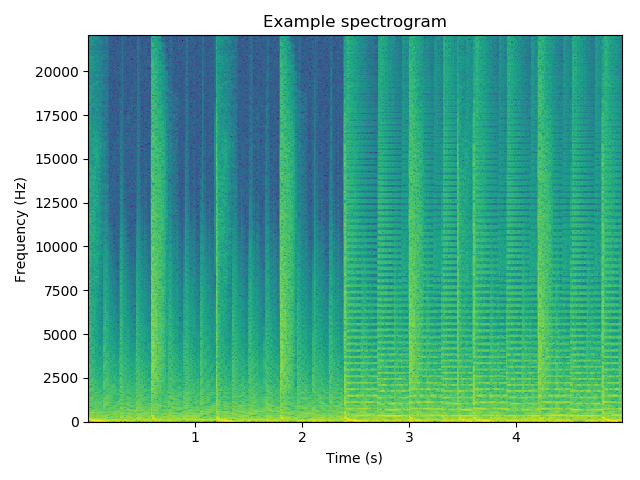
\includegraphics[width=\textwidth]{audio_specgram.png}
\end{figure}

Doing it this way will let us see how the frequency components change over time instead of taking the spectrum of the entire signal.

As with regular Fourier transform, we'll need to window each segment of the signal, but there is a caveat. Since we have windowed segments, we may be losing some information at the edge of each segment leading to artifacts, and furthermore we may be losing information about transients. To solve this, we'll need to introduce overlapping windows - however, having an overlap will increase the amount of coefficients required.

The continuous version is defined as: \cite{Recoskie2014ConstrainedNM}

\begin{align}
S(\tau, \xi) = \int_{-\infty}^{\infty}x(t)w(t-\tau)e^{-2\pi it\xi}dt
\end{align}

where $w$ is the window function.

But again, as we have discrete samples, we will need to use a discrete short-time Fourier transform, specifically:

\begin{align}
S_{k, \xi} = \sum_{n=-\infty}^{\infty}x_nw_{n-k}e^{-2\pi i\xi n}
\end{align}

And similarly to the regular Fourier Transform, short-time Fourier Transform is also invertible. \cite{selesnick_2009}

STFT is commonly used for audio analysis (e.g. for generating spectrograms) but in this case it will be used as a means for our NMF compression.

\subsubsection{Modified discrete cosine transform}
Modified discrete cosine transform, or MDCT for short, has become the dominant means of lossy high-quality audio coding. \cite{wang_vilermo_2012_mdct}

It is what's known as a \emph{lapped transform}. This means that when transforming a block into its MDCT coefficients, the basis function overlaps the block's boundaries. \cite{Malvar:1992:SPL:531523} In practice, what this means is that while we have blocks with overlapping windows as in the short-time Fourier transform, the number of coefficients remains the same as without while retaining the relevant properties.

As the name suggests, MDCT is based on the Discrete cosine transform, namely \emph{DCT-IV}, where the main difference is the addition of lapping mentioned above.

What makes MDCT simpler to work with compared to Fourier transform is that not only do we not need more coefficients despite overlapping, they are also real numbers as opposed to complex numbers, lowering the amount of bytes necessary to store them.

It is a linear function $f: \mathbf{R}^{2N} \rightarrow \mathbf{R}^N$, defined as: \cite{Babu2013FastAE}

\begin{align}
M_k = \sum_{n=0}^{N-1} x_n \cos \left\lbrace \frac{(2n+1+ \frac{N}{2} )(2k+1)\pi }{2N} \right\rbrace
\end{align}

for $k = 0, 1, \ldots, \frac{N}{2}-1$.

It is assumed that $x(n)$ is already windowed by an appropriate windowing function $w$.

MDCT is also invertible, and its inversion is defined as:

\begin{align}
\bar{x}_n &= \sum_{k=0}^{\frac{N}{2}-1} M_k \cos \left\lbrace \frac{(2n+1+ \frac{N}{2} )(2k+1)\pi }{2N} \right\rbrace
\end{align}

for $n = 0, 1, \ldots, N-1$.

It's important to note that the inverted transformed sequence $\bar{x}_n$ by itself does not correspond to the original signal $x_n$ \cite{prince_1986_tdac_1}. To achieve perfect invertibility, we must add subsequent overlapping blocks of the inverted MDCT (IMDCT). This method is called \emph{time domain aliasing cancellation} \cite{prince_1986_tdac_2}, or TDAC for short. As the name suggests, it mainly helps remove artifacts on the boundaries between transform blocks.

\section{Psychoacoustics}
Apart from time-frequency representations being generally more compact, they also give us the ability to analyse, isolate or modify the frequency composition of a given signal. This comprises a large chunk of the audio compressing process.

The field of psychoacoustics studies sound perception - that is, how our ears work and how we perceive different kinds of sounds. There are many different characteristics to sound that need to be taken into account for a proper psychoacoustic analysis \cite{olson1967music}, split into several categories, namely:

\begin{description}
	\item[tonal] includes pitch, timbre, melody harmony
	\item[dynamic] based on loudness
	\item[temporal] involves time, duration, tempo and rhythm
	\item[qualitative] represents harmonic constitution of the tone
\end{description}

For music, it's important to balance these four qualities appropriately. For compression, the most important qualities for us in scope of this work are going to be tonal (pitch) and dynamic (loudness).

\subsection{Pitch}
Pitch is a characteristic that comes from a frequency. The difference between the two is that pitch is our subjective perception of the tone whereas a frequency is an objective measure. Despite this fact, pitch is often quantified as a frequency using Hertz as its unit.

The lower bound of human hearing is around 20 Hz whereas the upper bound is most commonly cited as 20 000 Hz, or 20 kHz. \cite{rosen1993hearing} In a laboratory environment, people have been found to hear as low as 12 Hz. As people age, our hearing gets progressively worse and a healthy adult younger than 40 years can generally perceive frequencies only up to 15 kHz. \cite{olson1967music}

The human ear is capable of distinguishing different frequencies fairly accurately, though accuracy gets lower with increasing frequency. It's easier for our ears to tell a difference between 500 Hz and 520 Hz compared to the difference between 5000 Hz and 5020 Hz. \cite{smacdon_2018}

Furthermore, if we hear two different tones simultaneously, but their frequencies are close enough to one another, we may perceive them as a combination of tones rather than separate tones. Frequency ranges, or bands, where this phenomenon happens, are called \emph{critical bands}. \cite{fletcher_1940} It's also possible for one tone to mask the other entirely, and then we get what's called \emph{auditory masking}. \cite{gelfand1990hearing}

Based on the knowledge of the existence of these critical bands, it's possible to devise a system that specifies the range of each band in human hearing. One such scale that is commonly used is called the \emph{Bark scale}.

\subsubsection{Bark scale}
The Bark scale ranges from 1 to 24 Barks, where each Bark corresponds to a single critical band of human hearing. \cite{fastl_2006} The perceived difference in pitch between each band should be the same, despite the scale not growing linearly in terms of frequency ranges. Specifically, until around 500 Hz, the scale is roughly linear, but above that it has a more logarithmic growth. \cite{hermes_filter}

The Bark scale is commonly used as reference for audio encoding codecs, as we will see later. Knowledge of these critical bands allows for more educated byte allocation during the quantization process when compressing a frequency domain representation.

\begin{figure}[ht]
	\caption[Bark scale]{The Bark scale. Image by \href{https://commons.wikimedia.org/wiki/User:Swpb}{"Swpb"} licensed under \href{https://creativecommons.org/licenses/by-sa/4.0/deed.en}{CC BY-SA 4.0}.}
	\centering
	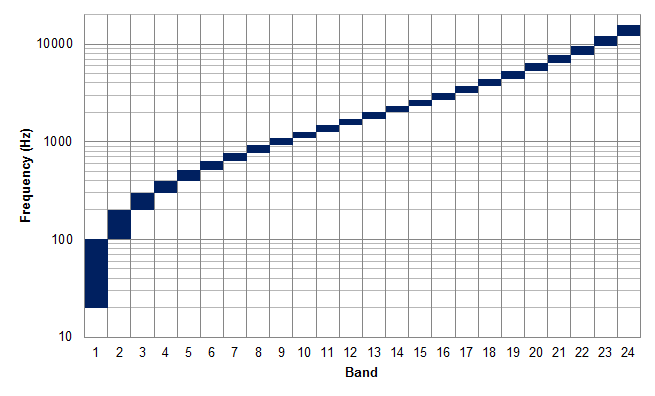
\includegraphics[width=\textwidth]{bark_scale.png}
\end{figure}

\subsection{Loudness}
What people often decide as loudness is really called \emph{sound pressure level} and it's measured in decibels (dB), however it has some shortcomings when it comes to psychoacoustic analysis.

It is defined as following: \cite{behar_1984}

\begin{align}
L_p = 20 \log_{10} \left( \frac{p}{p_0} \right) \text{dB}
\end{align}

where $p$ is a sound's sound pressure and $p_0$ is a reference sound pressure, also called the threshold of human hearing.

While this metric is very popular, it doesn't account for the fact that different frequencies have a different perceived loudness for a person's ears. \cite{olson1967music} There is a lot of research in recent years into how different frequencies impact our perception and hearing \cite{kuwano_1989}, but that is out of scope of this work. For more information about the exact definitions of loudness, refer to \cite{olson1967music}.

\subsection{Auditory masking}
As mentioned above, when it comes to audio masking, and therefore audio compression, we must not only take into account the critical bands as per e.g. the Bark scale, but also their intensity.

For example a lower frequency sound may mask one of a higher frequency, but the other way around does not apply. \cite{gelfand1990hearing} Modern audio encoders take this into account and using this knowledge are able to eliminate sounds that exist in the original signal, but are not perceivable by humans.

There are two important different kinds of masking effects - \emph{simultaneous} masking and \emph{temporal} masking. \cite{Raissi2002TheTB}

Simultaneous masking is what I have hinted at above - when there are two sounds within the same critical band, the dominant one may mask other frequencies within the same band. This can be compensated to a degree by increasing the volume of the masked sound.

Temporal masking does not occur in the frequency domain, but the time domain. The essence is that a stronger tonal component may mask a weaker one if they appear within a small window of time in succession.

\begin{figure}[ht]
	\caption[Auditory masking]{A hypothetical example of how a masker can shift the hearing threshold of a signal by 16 dB. Image created by \href{http://www.highprogrammer.com/alan/}{Alan De Smet} and published in the public domain.}
	\centering
	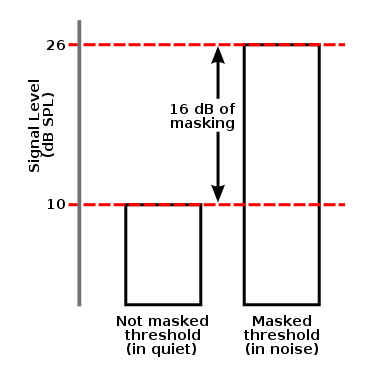
\includegraphics[width=0.7\textwidth]{auditory_masking.png}
\end{figure}


\chapter{Non-negative matrix factorization}
In today's age of big data, machine learning and various other fields, it's important to have ways to quickly analyse these datasets and ideally find patterns within. Non-negative matrix factorization is one of the paradigms suitable for that task.

\section{Linear dimensionality reduction}
Non-negative matrix factorization, or NMF, falls under \emph{linear dimensionality reduction} techniques. These are used widely for noise filtering, feature selection or compression, among others.

LDR can be defined as following: \cite{nmf_why_how}

\begin{align}
x_j &\approx \sum_{k=1}^{r}w_kh_j(k) &\text{for some weights $h_j \in \mathbf{R}^r$}
\end{align}

where given a data set of size $n$, we define $x_j \in \mathbf{R}^p$ for $1 \leq j \leq n$, $r < \min(p,n)$, and $w_k \in \mathbf{R}^p$ for $1 \leq k \leq r$.

What this effectively means is that we represent $p$-dimensional data points in a $r$-dimensional linear subspace, with basis elements $w_k$ and data coordinates given by vectors $h_j$. LDR defined in this manner is equivalent to low-rank matrix approximation, which is the essence of non-negative matrix factorization.

\section{NMF definition}
Non-negative matrix factorization solves the following NP-hard problem:

Given a non-negative matrix $V$, find non-negative matrix factors $W$ and $H$ such that:

\begin{align}
V \approx WH
\end{align}

That is, given a set of multivariate $n$-dimensional data vectors, we place these vectors in the columns of a $n \times m$ matrix $V$, where $m$ is the amount of examples we have. We then approximately factorize this matrix into two different matrices: a $n \times r$ matrix $W$ and a $r \times m$ matrix $H$. We generally choose $r < \min(n,m)$ (though this is not required) so that the two matrices are smaller than the original matrix $V$, essentially compressing it. \cite{nmf_algorithms}

\section{Classification}
NMF is as of currently still a relevant research topic, and has been explored by researchers from many different fields including mathematicians, statisticians, computer scientists or biologists. Given the wide range of use, over time it lead to different variations and additional constraints on the algorithms. Therefore, a taxonomy system was proposed in \cite{wang_zhang_2013}, outlined below.

.. TODO diagram of NMF categorization ..

\subsection{Basic NMF}
This is the basic model which only enforces non-negativity, and which all the following ones build upon.

However, due to its unconstrained nature, without any other constraints there are many possible solutions  which may lead to the algorithm's performance to vary. Further constraints outlined below help in the search of unique solutions.

\subsection{Constrained NMF (CNMF)}
Constrained NMF imposes additional constraints on the resulting matrices, namely:

\begin{description}
	\item[Sparse NMF] SPNMF, sparseness constraint
	\item[Orthogonal NMF] ONMF, orthogonality constraint
	\item[Discriminant NMF] DNMF, couples discriminant information along with the decomposition
	\item[NMF on manifold] MNMF, preserves local topological properties
\end{description}

\subsection{Structured NMF (SNMF)}
Structured NMF modifies standard factorization formulations:

\begin{description}
	\item[Weighed NMF] WNMF, attaches weights to different elements relative to their importance
	\item[Convolutive NMF] CVNMF, considers time-frequency domain factorization
	\item[Non-negative Matrix Trifactorization] NMTF, decomposes the data into three matrices
\end{description}

\subsection{Generalized NMF (GNMF)}
Generalized NMF can be considered a broader variant of Basic NMF, where conventional data types or factorization modes may be replaced with something different. It's split as follows:

\begin{description}
	\item[Semi-NMF] relaxes the non-negativity constraint on a specific factor matrix
	\item[Non-negative Tensor Factorization] NTF, generalizes the model to higher dimensional tensors
	\item[Non-negative Matrix-set Factorization] NMSF, extends the data sets from matrices to matrix-sets
	\item[Kernel NMF] KNMF, non-linear model of NMF
\end{description}

\section{Properties}
The additional constraint of non-negativity is important, as results show that it leads to a natural higher sparseness in both the basis matrix ($W$) and the encoding matrix ($H$). Additionally, non-negativity leads to a parts-based representation, which is similar to how our brains are presumed to work, basically combining parts in an additive manner to form a whole instead of subtracting. \cite{nmf_parts_objects} This sparseness makes it even easier to further compress the resulting matrices, saving us more space.

However this isn't without any downsides. While the concept of adding parts together seems to make a lot of sense, there is an issue. Since NMF employs a holistic approach, the additive parts learned by it in an unsupervised mode only considers features on a global level, and does not allow for representation of spatially localized features. \cite{li_spatial_lnmf_2001}

So while on paper NMF might seem better than PCA or SVD for a parts-based representation, it only comes at a cost of increased complexity, and since both PCA and SVD have a more compact spectrum than NMF, we must consider if this is worth the trade-off. \cite{wang_zhang_2013}

\section{Algorithms}
For the purposes of this thesis, we will only consider algorithms for Basic NMF. While NMF has been widely used in sound analysis etc. as we'll see below, its use for audio compression specifically is rare and there are limited resources to provide insight into utilizing possible constraints, therefore we will only be using the standard version.

Finding a decomposition of a matrix $V$ into matrices $W$ and $H$ is an NP-hard problem, and as such, the resulting matrices are generally only approximated over a number of iterations of an optimization algorithm. What this means in practice is that it's likely a result we'll find is sub-optimal or a local minimum.

\subsection{Cost function}
When using iterative updates, in each step of the process we need to evaluate the quality of the approximation. The function that does this is called the \emph{cost function}, or \emph{objective function}.

There are two simple commonly used functions. Firstly, we can use squared Euclidean distance: \cite{pentti_pmf_1997}

\begin{align}
||A-B||^2 = \sum_{ij}(A_{ij} - B_{ij})^2
\end{align}

This is lower bounded by 0, which it only is equal to if $A = B$.

Another metric we can use is based on Kullback-Leibler divergence, and is defined as such: \cite{nmf_algorithms}

\begin{align}
D(A||B) = \sum_{ij} \left( A_{ij} \log \frac{A_{ij}}{B_{ij}} - A_{ij} + B_{ij} \right)
\end{align}

\subsection{Update rules}
With the cost function in place, we now need a function to apply each iteration to try and minimize the value of the cost function. It has been found that a good compromise between speed and ease of implementation is to use what's called \emph{multiplicative update rules}. \cite{nmf_algorithms} Despite being over 15 years old, they are still very commonly used exactly for this reason.

For non-increasing Euclidean distance $||V - WH||$, if $W$ and $H$ are at a stationary point of distance, we may use these rules:

\begin{align}
H_{a \mu} & \leftarrow H_{a \mu} \frac{(W^TV)_{a \mu}}{(W^TWH)_{a \mu}} \\
W_{ia} & \leftarrow W_{ia} \frac{(VH^T)_{ia}}{(WHH^T)_{ia}}
\end{align}

And for non-increasing divergence $D(V||WH)$, if $W$ and $H$ are at a stationary point of divergence, we can use this:

\begin{align}
H_{a \mu} & \leftarrow H_{a \mu} \frac{\sum_i W_{ia} V_{i \mu} / (WH)_{i \mu}}{\sum_k W_{ka}} \\
W_{ia} & \leftarrow W_{ia} \frac{\sum_\mu H_{a \mu} V_{i \mu} / (WH)_{i \mu}}{\sum_v H_{av}}
\end{align}

.. TODO more update / cost functions used in music? ..

\section{Use in audio compression}
.. TODO paper128 ..

.. different kinds of nmf ..

.. use in audio ..


\chapter{Lossy audio compression}
Compression can be split into two kinds - lossy and lossless. Using "lossless" in the context of audio is a bit misleading, since sampling itself is a lossy process, but using a high enough sampling rate, we will not notice any difference, so sampled audio without any lossy compression will be our baseline.

For audio, lossless compression generally means taking some form of digital audio representation and losslessly compressing this data. This will preserve the signal in its entirety with a reduced bit-rate. However, due to size of such audio (an audio CD could only fit about 80 minutes of such music sampled at 44.1 kHz), it's become more common to use a lossy format.

Lossy compression implies that there will be loss of data, and while this is true, thanks to the application of various psychoacoustic principles size of audio can be greatly reduced without altering human perception, leading to vastly smaller bit-rates for no real cost.

This work focuses on lossy audio compression, therefore only lossy codecs will be considered for comparison.

\section{State of the art}
Due to its qualities of efficiently compacting energy and mitigating artifacts at block boundaries, MDCT is the most commonly used transformation in modern lossy audio coding, and is employed in the most popular audio formats including MP3, Opus, Vorbis or AAC.

In this section, I will elaborate on some of the more popular ones to get an idea of what considerations go into writing a modern audio codec.

\subsection{MP3}
.. TODO diagram ..

MP3, or MPEG-1 Layer III has been standardized in 1991 and has since become widespread throughout a multitude of electronic devices as the de-facto standard for music storage.

It's a very powerful compression/decompression scheme capable of reducing the bit-rate of an audio stream by up to a factor of 12 without any noticeable (to humans) quality degradation. In other words, to transmit CD quality audio, it needs a bitrate of 128 kbps. \cite{Raissi2002TheTB}

The core of MP3 compression is the Modified discrete cosine transform. The signal represented in its PCM form is first split into 32 subbands using an analysis polyphase filterbank, and each of those is further split into 18 MDCT bins, so overall we end up with 576 MDCT frequency bins per frame.

These bins are then sorted into 22 scalefactor bands, which roughly correlate to the 24 bands of human hearing. The point of these bands is that you may individually scale each of them up or down depending on how much precision you need for that specific frequency range. This usually done by dividing and rounding the values in the band, losing a certain amount of information; this process will be reversed during decoding.

The signal is also analyzed using the Fourier transformation, which gives us frequency information for the signal in the same frame, and we can use this information to determine how much to scale each scalefactor band - e.g. if there's some weak sound that will be masked by another, we can assign the band it's in lower precision, saving data. \cite{wilburn_2007}

Once we have the scaled and quantized data, we use the Huffman encoding to losslessly compress these values, and format this output into the final bitstream, encoding our audio.


\subsection{Opus (CELT)}
.. TODO diagram ..

.. how does it work ..

\part{Audio compression using NMF}
\chapter{Design}
In this chapter I will give an overview of how this audio codec will be designed, and explaining the various decisions I made along the way.

I have decided to call this new codec \emph{ANMF} (stands for Audio-NMF), using files with the extension \emph{.anmfx}, where \emph{x} represents the compression method. It will be implemented as a command line utility.

There are currently three different ANMF formats that you can choose from, and their main difference is which audio representation is being compressed by NMF. They are as follows:

\begin{description}
	\item[ANMF-RAW] denoted by \emph{r}, compresses the signal in PCM form (time domain)
	\item[ANMF-MDCT] denoted by \emph{m}, compresses the signal transformed with MDCT (frequency domain)
	\item[ANMF-STFT] denoted by \emph{s}, compresses the signal transformed with STFT (frequency domain)
\end{description}

\section{WAVE file}
WAVE, WAV or Waveform audio is a file format for storing digitized audio, created as a joint design by the Microsoft Corporation and the IBM Corporation. They are built on top of the chunk-based RIFF format. For details on the specific structure of a WAVE file please refer to \cite{sapp_pcm}.

It stores raw uncompressed audio samples in PCM format along with some metadata and will serve as both the standard input and output to the ANMF codec. Most commonly used formats can be converted to and from WAV as well and thus it will serve as a good baseline.

Samples in this format can be represented by different datatypes, I chose 16-bit signed integers, i.e. each sample's amplitude is represented by a whole number between $-32768$ and $32767$. The sample rate can vary, but a good standard value the experiments will use is $44.1$ kHz, which corresponds to audio CD quality.

\section {ANMF File structure}
The base container for the compressed ANMF file is the same no matter which encoding method you use. The bytes are saved in little endian byte order.

Please refer to Table \ref{tab:anmf_file} and each encoding method's table for the specific file structure. The first eleven bytes are mostly set in stone other than the method specification, but after that it varies greatly.

\begin{table}[htbp]\caption{ANMF file structure}
	\label{tab:anmf_file}
	\centering
	\begin{tabular}{|c|c|l|}
		\hline
		Bytes & Data type & Description \\ \hline
		0-3 & char[] & identifier string "ANMF" \\
		4 & char & method used, can be 'S', 'R' or 'M' \\
		5-6 & uint16 & \# of channels \\
		7-10 & uint32 & sample rate \\
		11-? & enc\_data & encoded data depending on the method \\
		\hline
	\end{tabular}
\end{table}

When serializing matrices to a file, the structure in Table \ref{tab:anmf_serial_matrix} will be used, denoted by a "matrix($dt$)" datatype in the following tables, where $dt$ stands for the datatype used for the matrix elements.

\begin{table}[htbp]\caption{Serialized matrix structure}
	\label{tab:anmf_serial_matrix}
	\centering
	\begin{tabular}{|c|c|l|}
		\hline
		Bytes (relative) & Data type & Description \\ \hline
		0-3 & uint32 & amount of rows in the matrix \\
		4-7 & uint32 & amount of columns in the matrix \\
		8-($8+x-1$) & $dt$ & row-wise values of the matrix, $x = rows*columns$ \\
		\hline
	\end{tabular}
\end{table}

There's also one more kind of matrix, a matrix using Huffman encoded quantized values. This will be denoted by a "quant\_matrix" datatype. For its specification please see Table \ref{tab:anmf_serial_quant_matrix}.

\begin{table}[htbp]\caption{Serialized quantized matrix structure}
	\label{tab:anmf_serial_quant_matrix}
	\centering
	\begin{tabular}{|c|c|l|}
		\hline
		Bytes (relative) & Data type & Description \\ \hline
		0-3 & uint32 & amount of rows in the matrix \\
		4-7 & uint32 & length $L$ of the Huffman encoded byte stream \\
		8-($8+L-1$) & byte[] & Huffman encoded byte stream representing the matrix \\
		\hline
	\end{tabular}
\end{table}

\section{Encoder}
The encoder is responsible for taking a raw audio file and encoding the data within, producing a compressed version of the original. Please refer to Figure \ref{fig:design_encoder} for a visual representation of the process.

\begin{figure}[ht]
	\caption[Encoder overview]{A high level overview of the ANMF audio encoder.}
	\label{fig:design_encoder}
	\centering
	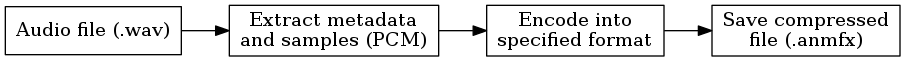
\includegraphics[width=\textwidth]{design_encoder.png}
\end{figure}

Next, each format's encoding process will be outlined (third step in the figure). If the audio file has multiple channels, this process is repeated on each channel separately.

\subsection{ANMF-RAW}
\begin{figure}[ht]
	\caption[ANMF-RAW Encoder]{The encoding scheme for ANMF-RAW.}
	\label{fig:encoding_nmf_raw}
	\centering
	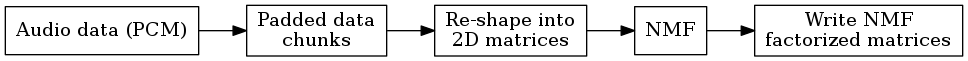
\includegraphics[width=\textwidth]{nmf_raw.png}
\end{figure}

ANMF-RAW works on the principle of applying NMF directly to the PCM audio samples $x_n$. However, the samples are initially an array of 16-bit signed integers, and as such, they need to be processed first before NMF can be used.

A chunk shape is specified to determine how many rows and columns each matrix will have before NMF. We choose a target matrix shape of $1152 \times 200$ to match the amount of samples per frame in the other methods.The sample array is then padded with zeroes to ensure there are enough elements at the end of the array to ensure every matrix can have the same shape and number of elements. The amount of padding must be written to the output so that we know the length of the original array when decoding.

Once the array is padded, we iterate over the samples and split them into equal chunks of size $rows*columns$. This array is then "folded" to produce a matrix of the desired shape. We then obtain a matrix of signed integers, so in order to be able to use NMF, we first need to get rid of all the negative values. To do that, we increment each chunk by the absolute value of its smallest element, guaranteeing that the lowest value in the matrix is $\ge 0$.

Once we have this matrix, we proceed by applying basic random-initialized Euclidean-based NMF on it, obtaining the basis matrix $W$ and coefficient matrix $H$. Lastly, for each chunk, we write the value we incremented the matrix by, and the two decomposition matrices.

\begin{table}[htbp]\caption{ANMF-RAW data structure}
	\label{tab:anmf_raw_file}
	\centering
	\begin{tabular}{|c|c|l|}
		\hline
		Bytes (relative) & Data type & Description \\ \hline
		0-3 & uint32 & amount of zeroes used to pad the samples \\
		4-7 & uint32 & amount of chunks \\
		8-? & data\_chunk[] & NMF-compressed data chunks (refer to Table \ref{tab:anmf_raw_data}) \\
		\hline
	\end{tabular}
\end{table}

\begin{table}[htbp]\caption{ANMF-RAW structure of each data chunk}
	\label{tab:anmf_raw_data}
	\centering
	\begin{tabular}{|c|c|l|}
		\hline
		Bytes (relative) & Data type & Description \\ \hline
		0-7 & float64 & absolute value that the matrix was incremented by \\
		8-? & matrix(float32) & matrix $W$ \\
		?-? & matrix(float32) & matrix $H$ \\
		\hline
	\end{tabular}
\end{table}

\subsection{ANMF-MDCT}
\begin{figure}[ht]
	\caption[ANMF-MDCT Encoder]{The encoding scheme for ANMF-MDCT.}
	\label{fig:encoding_nmf_mdct}
	\centering
	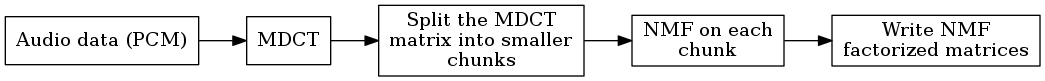
\includegraphics[width=\textwidth]{nmf_mdct.png}
\end{figure}

In ANMF-MDCT, as the name suggests, the PCM input will be transformed using MDCT as per Section \ref{sec:mdct}. Since this is a lapped transform, each transformed block will have a 50\% overlap with the following block. We choose a frame size of $2N = 1152$ and split the signal into blocks of that size, thus each block will contain $N = 576$ coefficients from its own block, and another $576$ from the following one.

The decision to have a block size of $N = 576$ stems from the fact that this will give us the same amount of frequency resolution that e.g. MP3 uses (as seen in Section \ref{sec:mp3}), which proved to be enough for human hearing.

As before, we first pad the signal at the end with zeroes to align it to the desired block size. To prevent loss of data in the first and the last block due to the overlapping, we further pad the signal by an array of zeroes, equal in size to the size of a block, that is $N$ zeroes both at the beginning and the end of the signal.

Then, we apply a windowing function on each block to bring the values near the edges closer to $0$ to help mitigate spectral leakage. We use the MLT window $w_n^M$ as defined in Section \ref{sec:mlt}.

Finally, we apply the MDCT on each of the windowed blocks and obtain a matrix of MDCT coefficients in the form of real numbers.

This matrix is then split into smaller chunks. For example, if the MDCT matrix contains $576$ rows and $1100$ columns, we might split it into submatrices sized $576 \times 200$, with the last one being $576 \times 100$, as no padding is necessary here. This amount of chunks is written to the output. Basic random-initialized Euclidean-based NMF is then ran on each of the chunks separately and the decomposition matrices serialized.

\begin{table}[htbp]\caption{ANMF-MDCT data structure}
	\label{tab:anmf_mdct_file}
	\centering
	\begin{tabular}{|c|c|l|}
		\hline
		Bytes (relative) & Data type & Description \\ \hline
		0-3 & uint32 & amount of zeroes used to pad the samples \\
		4-7 & uint32 & amount of MDCT submatrix chunks \\
		8-? & data\_chunk[] & NMF-compressed MDCT chunks (refer to Table \ref{tab:anmf_mdct_data}) \\
		\hline
	\end{tabular}
\end{table}

\begin{table}[htbp]\caption{ANMF-MDCT structure of each data chunk}
	\label{tab:anmf_mdct_data}
	\centering
	\begin{tabular}{|c|c|l|}
		\hline
		Bytes (relative) & Data type & Description \\ \hline
		0-7 & float64 & absolute value that the matrix was incremented by \\
		8-? & matrix(float32) & matrix $W$ \\
		?-? & matrix(float32) & matrix $H$ \\
		\hline
	\end{tabular}
\end{table}

\subsection{ANMF-STFT}
\begin{figure}[ht]
	\caption[ANMF-STFT Encoder]{The encoding scheme for ANMF-STFT.}		\label{fig:encoding_nmf_stft}
	\centering
	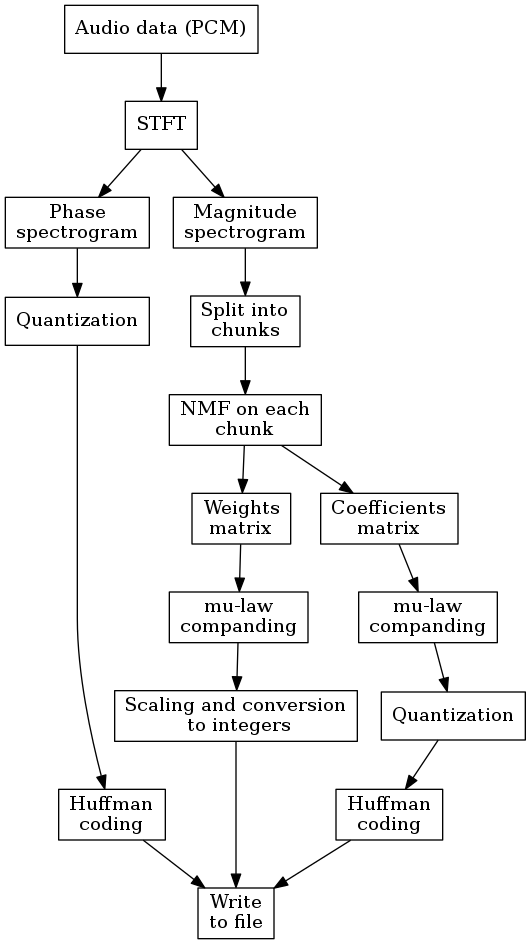
\includegraphics[width=0.6\textwidth]{nmf_stft.png}
\end{figure}

The design of ANMF-STFT is based on the solution suggested in \cite{nikunen_2010} with some changes along with only utilizing open source solutions.

Like with ANMF-MDCT, we choose a frame size of $N = 1152$, leading to a frequency resolution of $576$ bins. We begin by properly padding the signal to $N$ so that it's possible to be split into equal parts. We then use STFT with 50\% overlap and a block size of $N$, which means we end up with twice the coefficients compared to MDCT, but this is not a major issue.

During STFT, we must again window each block, leading to overlapping windows. We use the Hann window $w_n^H$ for this (as defined in Section \ref{sec:hann}).

Once STFT is finished, we end up with a matrix of Fourier transform coefficients in the form of complex numbers. Trying to apply NMF on the complex numbers directly would yield similar results to ANMF-MDCT, so we have to approach this differently.

If we visualise the complex valued elements in the complex plane, we can instead represent each element $z$ as two separate values:

\begin{description}
	\item[magnitude] also called the modulus, geometrically it's the distance from 0
	\item[phase] also called the argument, geometrically it's the angle from the real axis
\end{description}

To obtain the phase $\phi$ of a complex number $z = x + iy$, we can use the following formula:

\begin{align}
\phi(z) = \arg(z) = \arctantwo(y,x)
\end{align}

And to obtain the magnitude $|z|$ of the complex number:

\begin{align}
|z| = \sqrt{x^2 + y^2}
\end{align}

By calculating the magnitude and phase of every element in the STFT matrix individually, we obtain the magnitude spectrogram and the phase spectrogram respectively. We now need to encode both of them individually.

For the phase matrix, my experiments showed that applying NMF on it leads to a very noticeable loss in quality, so instead I opted for a different solution that ultimately ends up saving more space than NMF would.

The phase matrix contains values ranging from $-\pi$ to $\pi$. These values are uniformly quantized into 8 levels ($n_p = 3$ bits) as per Section \ref{sec:unif_quant}. Due to the relative frequency of the boundary values $-\pi$ and $\pi$, a mid-tread quantizer is used. The frequency of each quantization level is visible in Figure \ref{fig:stft_phase_quant_freq}.

Using these frequencies, we are able to then construct a Huffman coding table (refer to Section \ref{sec:huffman}) and use it to losslessly encode the quantized phase matrix using at most 4 bits per value.

\begin{figure}[ht]
	\caption[ANMF-STFT quantized phase frequencies]{Frequency of each quantization level in the phase spectrogram. Data taken from the average of all the example audio files.}
	\label{fig:stft_phase_quant_freq}
	\centering
	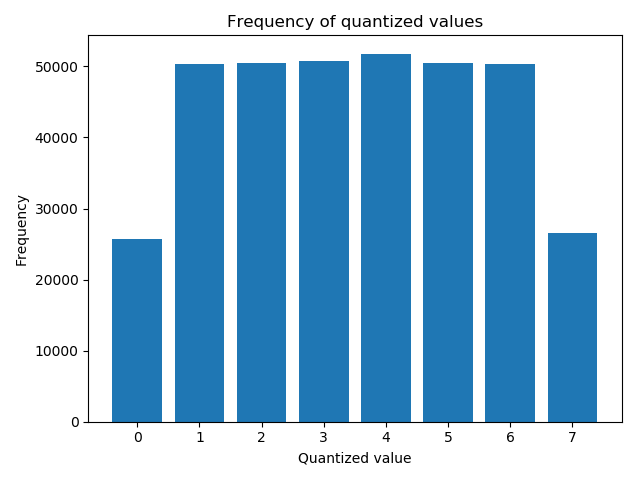
\includegraphics[width=\textwidth]{stft_phase_quant_freq.png}
\end{figure}

The magnitude spectrogram is where we actually use NMF. As it is effectively a matrix of signal amplitudes, it's less prone to noticeable quality loss if the values deviate a little. We split the magnitude matrix column-wise into smaller submatrices, e.g. $chunk_size = 500$.

On each submatrix we then run basic random-initialized Euclidean-based NMF, obtaining the weight matrix $W$ and coefficient matrix $H$.

For the next step, we apply $\mu$-law compression to both the decomposition matrices, as defined in Section \ref{sec:mulaw}. In order to be able to do that, we first scale both matrices to the range $[0, 1]$. We do this by applying the following formula to all elements in both matrices:

\begin{align}
M'_{ij} = \frac{M_{ij} - \min(M)}{|\max(M) - \min(M)|}
\end{align}

To restore the original scale later, we need to save both the minimum and maximum value, otherwise they will be lost in the non-uniform quantization.

For the $\mu$-law compression, we experiment with the value of $\mu$ later, but a good start is $\mu_W = 10^4$ and $\mu_H = 10^5$. We do this because we want to lower the amount of bits needed to represent each value, without losing the values near zero - that would lead to a large loss of quality, or in some cases, loss of the signal itself.

In the weight matrix, we then convert the compressed values into 32-bit unsigned integers, as going to values below that proved to cause loss of signal data, and this integer matrix is then serialized into the file.

However, in the case of the coefficient matrix $H$, we can go a lot further. We use a uniform quantizer with 32 levels ($n_h = 5$ bits) and we opt for a mid-tread quantizer again, as we want to be able to reconstruct a value of $0$, i.e. feature not present.

Similarly to the phase matrix, we take these quantized values and look at their frequencies. The results of this analysis are visible on Figure \ref{fig:stft_quant_freq}.

\begin{figure}[ht]
	\caption[ANMF-STFT quantized magnitude coefficient frequencies]{Frequency of each quantization level in the decomposed coefficients matrix of the magnitude spectrogram. Data taken from the average of all the example audio files.}
	\label{fig:stft_quant_freq}
	\centering
	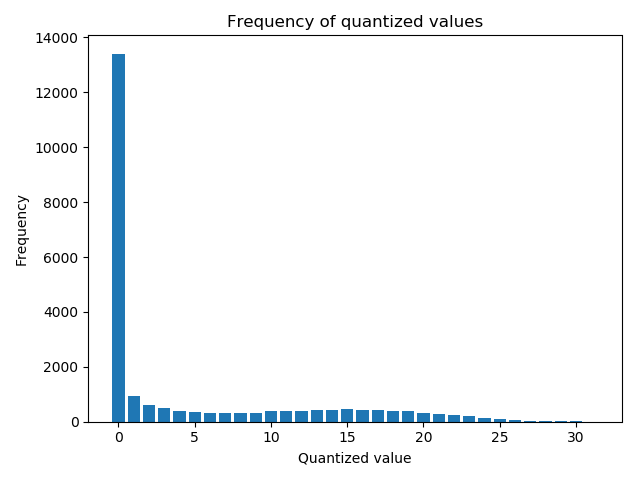
\includegraphics[width=\textwidth]{stft_quant_freq.png}
\end{figure}

Using this information, we can construct another Huffman coding table, separate for this matrix. As we can see, even despite the $\mu$-law compression, a lot of values still fall to a quantized value of $0$.

In a Huffman table from these frequencies, we then assemble the shortest code to the value $0$, i.e. we only need 1 bit. The longest code in a table constructed this way for 32 levels of quantization will only require 11 bits. Overall, we save a lot of space saving the matrix this way as opposed to storing the values as 32-bit floats or integers.

\begin{table}[htbp]\caption{ANMF-STFT data structure}
	\label{tab:anmf_stft_file}
	\centering
	\begin{tabular}{|c|c|l|}
		\hline
		Bytes (relative) & Data type & Description \\ \hline
		0-3 & uint32 & amount of zeroes used to pad the samples \\
		4-7 & uint32 & amount of STFT submatrix chunks \\
		8-? & quant\_matrix & quantized phase matrix \\
		?-? & data\_chunk[] & NMF-compressed magnitude chunks (refer to Table \ref{tab:anmf_stft_data}) \\
		\hline
	\end{tabular}
\end{table}

\begin{table}[htbp]\caption{ANMF-STFT structure of each magnitude submatrix}
	\label{tab:anmf_stft_data}
	\centering
	\begin{tabular}{|c|c|l|}
		\hline
		Bytes (relative) & Data type & Description \\ \hline
		0-7 & float64 & absolute value that the matrix was incremented by \\
		8-15 & float64 & minimum value before scaling to $[0, 1]$ \\
		16-23 & float64 & maximum value before scaling to $[0, 1]$ \\
		24-? & matrix(uint32) & $\mu$-law compressed matrix $W$ \\
		?-? & quant\_matrix & quantized $\mu$-law compressed matrix $H$ \\
		\hline
	\end{tabular}
\end{table}

\subsubsection{Huffman encoding}
\label{sec:huffman}
Huffman code refers to an optimal prefix coding scheme often employed for lossless compression. It's used to compress a message that only consists of members from a finite, known beforehand set of symbols. \cite{huffman_1952}

The goal is to create a dictionary that maps each value to a sequence of bits, where none of the sequences is a prefix of another one, which means that there are no ambiguities when decoding a Huffman encoded message, and we do not need to store any information about where one code begins and where it ends.

The main characteristic of a Huffman code is that the more frequent a symbol is, the shorter code it will be assigned. So in the case of a system where a certain symbol is very frequent, a message consisting of mostly those symbols will be compressed greatly, with no loss of data.

\begin{algorithm}[h]
\caption{Huffman code compression}
\label{alg:huffman}
\KwIn{a list of symbols and their probabilities}
\KwOut{a Huffman tree}
queue $\leftarrow$ new PriorityQueue()\;
\ForEach{item x in input}{
	node $\leftarrow$ new Node()\;
	node.symbol $\leftarrow$ x.symbol\;
	node.prob $\leftarrow$ x.probability\;
	node.leftChild, node.rightChild $\leftarrow$ null\;
	queue.enqueue(node, node.prob)\;
}
\While{queue.length $>$ 1}{
	node1 $\leftarrow$ queue.dequeue()\;
	node2 $\leftarrow$ queue.dequeue()\;
	newNode $\leftarrow$ new Node()\;
	newNode.leftChild $\leftarrow$ node1\;
	newNode.rightChild $\leftarrow$ node2\;
	newNode.prob $\leftarrow$ node1.prob + node2.prob\;
	queue.enqueue(newNode, newNode.prob)\;
}
\end{algorithm}

Algorithm \ref{alg:huffman} describes the compression process, at the end of which we obtain a Huffman tree. By traversing this tree from the root and assigning every left child a $0$ and every right child a $1$ and concatenating these bits as we reach the symbols in the leafs, we obtain the Huffman code for the given symbol. The asymptotic complexity of this algorithm is $\mathcal{O}(n \log n)$, essentially we need $\mathcal{O}(\log n)$ time to determine the highest priority in the queue, and there are $\mathcal{O}(n)$ iterations.

Often, the dictionary itself has to be encoded as well, but as the frequencies are roughly the same for each audio file, the tree can be fixed directly into the implementation.

\section{Decoder}
Similar to the encoder, the decoder simply reverses the encoding process as seen in Figure \ref{fig:design_decoder}. As this process is fairly straightforward for each of the methods, it won't be elaborated on further.

\begin{figure}[ht]
	\caption[Decoder overview]{A high level overview of the ANMF audio decoder.}
	\label{fig:design_decoder}
	\centering
	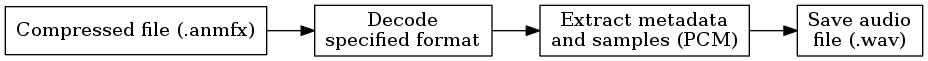
\includegraphics[width=\textwidth]{design_decoder.png}
\end{figure}


\chapter{Implementation}
This chapter will explain the specific details of implementing the audio codec outlined in the previous chapter.

\section{Encoder}
.. process of encoding ..

\subsection{NMF-RAW}
TODO

\subsection{NMF-MDCT}
TODO describe MDCT as transformed DCT-IV (mdct.py)

\subsection{NMF-STFT}

.. application of NMF ..

.. variables ..

\section{Decoder}

\chapter{Evaluation}
In this section you will find an evaluation of the different algorithms, including experiments with various parameters for them and comparison to existing solutions from Section \ref{sec:stateoftheart}.

\section{Methodology}
Audio compression quality is most often evaluated using a series of listening tests (such as the one pictured in Figure \ref{fig:opus_listening_test}). However, due to a lack of resources to conduct such a thing, a different method must be used - although they are generally not as accurate.

One of the most used methods for objectively evaluating perceptible audio quality is PEAQ \cite{peaq_2006}, however its specifications are insufficient, and its implementations proprietary. The exact algorithm and parameters aren't known for the most part. It comes in two variants:

\begin{description}
	\item[PEAQ Basic] intended for real-time use
	\item[PEAQ Advanced] a more comprehensive model, intended for non real-time use
\end{description}

Even though neither of these is directly available, luckily, there are a few open-source alternatives that try to implement similar algorithms, with their quality measured by comparing their output to PEAQ, and by proxy, to listening tests.

One of the more prominent open-source solutions is GstPEAQ, which according to its paper \cite{gstpeaq_paper} performs better than the other implementations. So while it does not conform to the PEAQ recommendation directly, its results are within an acceptable margin and thus this thesis will use GstPEAQ for quality evaluation.

\section{GstPEAQ}
GstPEAQ is a plugin for GStreamer \cite{gstreamer_2016} (a pipeline-based multimedia framework) and its source code is freely available at \cite{gstpeaq_impl}. It implements both the Basic and Advanced mode of PEAQ as specified in \cite{peaq_2006}, however as the standard is under-specified, educated guesses must be taken at points.

And just like PEAQ, the algorithm's main output is a value known as \emph{Objective Difference Grade} (ODG), which evaluates the perceptible impairment (quality difference) between the provided audio and the reference audio. It uses various psychoacoustic "features" of the signal to determine the grade, the details of which won't be covered here - please refer to either paper for specifics.

The ODG scale contains real values from $0$ to $-4$, ranging from imperceptible difference to very annoying for the human ear. Please refer to Table \ref{tab:odg_scale} to see the full scale.

\begin{table}[htbp]\caption{PEAQ - Objective Difference Grade table}
	\label{tab:odg_scale}
	\centering
	\begin{tabular}{|c|l|}
		\hline
		ODG & Impairment description \\ \hline
		$0.0$ & Imperceptible \\
		$-1.0$ & Perceptible, but not annoying \\
		$-2.0$ & Slightly annoying \\
		$-3.0$ & Annoying \\
		$-4.0$ & Very annoying \\
		\hline
	\end{tabular}
\end{table}

\section{Evaluating results}
In this section we will experiment with various parameters for all the encoding methods, find a good compromise between bitrate and ODG, and then compare those results to the reference codings (MP3, Opus) at similar bitrates.

The evaluating process will work in these steps:

\begin{enumerate}
	\item compress example WAV file using ANMF
	\item decompress ANMF back to a WAV file
	\item measure ODG between old and new WAV file
\end{enumerate}

In the case of MP3 or Opus files, they will be decoded to WAV for comparison.

\subsection{Audio examples}
There's a total of four example audio files in WAV format that will be used for testing. Please refer to Table \ref{tab:audio_examples} for a list. All of the examples are $\sim5-10$ second excerpts from audio files using 44.1 kHz sampling rate and 16-bit signed integer samples. These files can be found in the \verb|examples| folder of the implementation.

\begin{table}[htbp]\caption{List of tested audio files}
	\label{tab:audio_examples}
	\centering
	\begin{tabular}{|c|c|c|c|l|}
		\hline
		ID & File name & Description \\ \hline
		$00$ & \verb|piano16t.wav| & Clear sounding piano sounds \\
		$01$ & \verb|henry16t.wav| & Average quality English voice \\
		$02$ & \verb|swave16t.wav| & Simple electronic music \\
		$03$ & \verb|taleena16t.wav| & Complex music including lyrics \\
		\hline
	\end{tabular}
\end{table}

\subsection{Bitrate}
The bitrate is the amount of bits that a computer needs to process per a unit of time, in this context it means how many bits are needed to play back 1 second of an audio file.

To find the bitrate of a WAV file, we can use the following equation:

\begin{align}
bitrate = channelCount \cdot samplingRate \cdot bitsPerSample
\end{align}

So in regards to compressing the example files, our target bitrate is at most $2 \cdot 44100 \cdot 16 = 1411200$ bits per second (or $\sim 1411$ kbps).

To calculate the number of elements in an NMF-approximated matrix $V$ of size $m \times n$ with approximation rank $r$, we can use the following equation:

\begin{align}
\label{equ:nmf_size}
size(NMF(V)) = r(m+n)
\end{align}

\emph{Proof:} NMF approximates a matrix $m \times n$ into two matrices $m \times r$ and $r \times n$, therefore the total size is $mr + rn = r(m+n)$.

\subsection{ANMF-RAW}
For ANMF-RAW, we need to find a compromise between the size of one chunk and the rank of the NMF. First, we'll fix the shape to $1152 \times 200$ and experiment with the rank.

The maximum number of iterations has been fixed to 3000, since past that point the cost function is almost stable as seen in Figure \ref{fig:anmf_raw_cost_func}.

\begin{figure}[ht]
	\caption[ANMF-RAW cost function]{The value of the cost function per iteration during NMF in ANMF-RAW at rank $= 30$.}
	\label{fig:anmf_raw_cost_func}
	\centering
	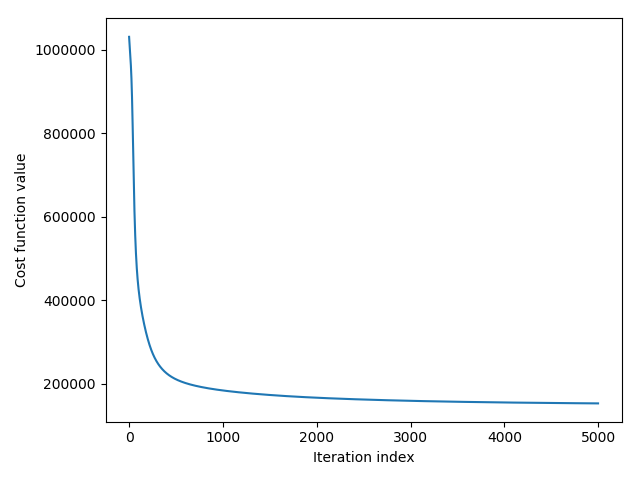
\includegraphics[width=\textwidth]{anmf_raw_cost_func.png}
\end{figure}

In Table \ref{tab:anmf_raw_rank}, you can see the results of changing the rank of the NMF approximation. The rows correspond to the example IDs from Table \ref{tab:audio_examples}, and the columns correspond to the ODG for different rank values.

\begin{table}[htbp]\caption{ANMF-RAW rank experiment results}
	\label{tab:anmf_raw_rank}
	\centering
	\begin{tabular}{|c|c|c|c|c|c|}
		\hline
		ID & rank 30 & rank 40 & rank 45 & rank 60 & rank 75 \\ \hline
		$00$ & $-3.873$ & $-3.830$ & $-3.811$ & $-3.749$ & $-3.650$ \\
		$01$ & $-3.908$ & $-3.902$ & $-3.895$ & $-3.861$ & $-3.844$ \\
		$02$ & $-3.868$ & $-3.850$ & $-3.837$ & $-3.800$ & $-3.759$ \\
		$03$ & $-3.744$ & $-3.519$ & $-3.361$ & $-2.825$ & $-2.461$ \\		
		\hline
	\end{tabular}
\end{table}

It's also worth mentioning that the runtime necessary for compression scales with the rank, as seen in Table \ref{tab:anmf_raw_runtime}.

\begin{table}[htbp]\caption{ANMF-RAW average runtime in seconds}
	\label{tab:anmf_raw_runtime}
	\centering
	\begin{tabular}{|c|c|c|c|c|c|}
		\hline
		ID & rank 30 & rank 40 & rank 45 & rank 60 & rank 75 \\ \hline
		$00$ & $63.378$s & $65.913$s & $67.082$s & $71.684$s & $75.839$s \\	
		\hline
	\end{tabular}
\end{table}

Interestingly enough, sample ID 03 notices the largest improvement despite being the more complex of the four, but when listening to the decompressed audio, it still sounds quite distorted and noticeable. Another looming issue is that at that rank the size of the compressed file approaches the original filesize, so we will need to lower the rank and try a lower chunk size instead.

To calculate the bitrate of ANMF-RAW, we must take into account the chunk size and the rank of the NMF approximation and then use Equation \ref{equ:nmf_size}. There is some overhead for the metadata, but as it spans only a few bytes it will be disregarded. The bitrate of ANMF-RAW with a chunk size of $m \times n$ and rank $r$ can be calculated as:

\begin{align}
bitrate^R = r(m+n) \cdot \frac{sampleRate}{mn} \cdot bitsPerValue \cdot channelCount
\end{align}

Therefore, for a chunk $1152 \times 200$ with rank 75, we get:

\begin{align}
bitrate^R = 75 \cdot (1152 + 200) \cdot \frac{44100}{1152 \cdot 200} \cdot 32 \cdot 2 = 1242150
\end{align}

Our target is 1411 kbps and our compression with 1242 kbps is judged as "annoying" by GstPEAQ. We will try lowering the chunk size and rank both to see if it has an effect. It was mentioned in Section \ref{sec:mp3} that it can compress music by up to a factor of 12 without noticeable loss in quality. Here, with this method, we are going to aim for at least around half that.

We take a rank of 40 and a target bitrate of 750 kbps. We pick e.g. $600$ for $m$ and solve the equation above, obtaining $n = 200$. However, when trying out these new parameters, the ODG barely changed from the previous shape, and further testing of this method was thus stopped due to unsatisfactory results.

\subsection{ANMF-MDCT}
.. TODO experiment with parameters and calculate bitrate ..

\subsection{ANMF-STFT}
.. TODO experiment with parameters and calculate bitrate ..

\subsection{Comparison}
.. TODO calculate bitrate for the wav files ..
.. TODO compare the "best" from the previous 3 vs MP3/Opus ..


\setsecnumdepth{part}
\chapter{Conclusion}
.. what went right ..


.. what went wrong ..


.. what could be improved ..
add psychoacoustics
try compressing LPC/SILK


\bibliographystyle{iso690}
\bibliography{mybibliographyfile}

\setsecnumdepth{all}
\appendix

\chapter{Acronyms}
\begin{description}
	\item[todo] TODO
\end{description}


\chapter{Contents of enclosed CD}

\begin{figure}
	\dirtree{%
		.1 readme.txt\DTcomment{the file with CD contents description}.
		.1 exe\DTcomment{the directory with executables}.
		.1 src\DTcomment{the directory of source codes}.
		.2 wbdcm\DTcomment{implementation sources}.
		.2 thesis\DTcomment{the directory of \LaTeX{} source codes of the thesis}.
		.1 text\DTcomment{the thesis text directory}.
		.2 thesis.pdf\DTcomment{the thesis text in PDF format}.
		.2 thesis.ps\DTcomment{the thesis text in PS format}.
	}
\end{figure}

\end{document}
